\documentclass[
  oneside,
  %twoside,
  11pt, a4paper,
  footinclude=true,
  headinclude=true,
  cleardoublepage=empty
]{scrbook}

\usepackage{dissertation}

% ACRONYMS -----------------------------------------------------
\usepackage[acronym,nonumberlist,nomain]{glossaries}

%enable the following to avoid links from the acronym usage to the list
\glsdisablehyper

\defglsdisplayfirst[\acronymtype]{\emph{#1#4}}

\glossarystyle{listgroup}

\renewcommand{\glossaryname}{Acronyms}

\makeglossaries

% Acronym entries -----------------------------------------
% S
\newacronym{sn}{SN}{Social Network}
\newacronym{sna}{SNA}{Social Network Analysis}
% O
\newacronym{osn}{OSN}{Online Social Network}

% ----------------------------------------------------------------

% Title
\titleA{Analysis and Visualisation of}
\titleB{Dynamic Social Networks}

% Author
\author{Jorge Caldas}

% Supervisor(s)
\supervisor{Pedro Rangel Henriques}
\cosupervisor{Alda Lopes Gan\c{c}arski}

% Date
\date{\myear}

% Keywords
%\keywords{master thesis}

% Glossaries & Acronyms
%\makeglossaries
%\makeindex	   % ... or this

% Define Acronyms
%%!TEX root = ../dissertation.tex

\newacronym{rest}{REST}{Representational State Transfer}
%\glsaddall[types={\acronymtype}]

\ummetadata

\newcommand{\itab}{\hspace{4em}}
\begin{document}
	% Cover page ---------------------------------------
	\umfrontcover
	\umtitlepage
	
	% Add acknowledgements ----------------------------
	\chapter*{Acknowledgements}
	Write acknowledgements here

	% Add abstracts (en,pt) ---------------------------
	\chapter*{Abstract}
	Write abstract here (en) or import corresponding file
	
	\cleardoublepage
	\chapter*{Resumo}
	Escrever aqui resumo (pt) ou importar respectivo ficheiro
	
	% Summary Lists ------------------------------------
	\tableofcontents
	
	\addtocontents{toc}{\protect\hypertarget{toc}{}}
	%\rfoot{\textit{\hyperlink{toc}{Social Networks}}}
	
	\listoffigures
	\listoftables
	%\lstlistoflistings
	%\listofabbreviations
	\printglossary[type=\acronymtype]
	\clearpage
	\thispagestyle{empty}
	
	\pagenumbering{arabic}
	
	% CHAPTER - Introduction -------------------------
	\chapter{Introduction}
	\section{Context and Problem}
	%SNs, SNA, OSNs, Unstructured Data Analysis
	\section{Motivation}
	% Many Analyse Unstructured Data means a lot of things that we can infer and dicover
	% the information is there and it is up to us to make good and creative use of it
	\section{Goals}
	% Analyse Unstructured Data
	
	
	% CHAPTER - Social Networks in Sociology -------------------------
	\chapter{Social Networks in Sociology}
	%% ---------------------------------------------- Chapter Introduction

\indent \indent Nowadays is hard to find something that is not organized as a network, if one tries to understand something about the world around us, then definitely one needs to know something about networks.

Curiously if you look up the term \textit{''social network''} in the Cambridge Dictionary, we may face the following:

\begin{quote}
\textit{"a website or computer program that allows people to communicate and share information on the Internet using a computer or mobile phone"}
\end{quote}
%\cite{cambridge_dict_sn}

But, even if today we automatically think in SNs as websites (or web applications), deep down we know when talking about SNs, we refer to a much more broader term, that said, we may consider a SN as the following:

\begin{quote}
\textit{"A social structure made of nodes that are generally individuals or organizations. A social network represents relationships and flows between people, groups, organizations, animals, computers or other information/knowledge processing entities. The term itself was coined in 1954 by J. A. Barnes."}
\end{quote}
%\cite{webopedia_sn_defenition}

One may say that networks work like pipes, and trough them things flow, from individual to individual inside the network. It's trough networks that big institutions can organize themselves, and actually add value to society despite the large number of individuals.

%% ---------------------------------------------- Origins of Social Networks
\section{Origins of Social Networks}

\begin{quote}
\textit{''The network concept is one of the defining paradigms of the modern era.''} [REF\_BOOK]
\end{quote}

\indent Before talking of network from the sociology perspective, one needs to review the network concept, which is broadly used across multiple fields of study, this include, physics, biology, linguistic, anthropology, mathematics, computer science and more recently computer networks.

\indent But why is the network approach so adopted in such diversification fields? The answer is, because networks allows us to capture the interactions of any individual unit within the larger field of activity to which the unit belongs [REF\_BOOK].


\subsection{Sociology Perspective}
\begin{quote}
\textit{"(...) many people attribute the first use of the term ''social network'' to
Barnes (1954). The notion of a network of relations linking social entities, or of webs or ties among social units emanating through society, has
found wide expression throughout the social sciences. (...)"}
\end{quote}
%\cite{sna_bible}

The \textit{''social network''} concept has been around for many years now, maybe not in the exact format that nowadays, we are familiarized with (''\textit{web way}'', in a manner of speaking), but in a more abstract sense, applied in real life within real connections.
In \textit{"Social Network Analysis - Methods and Applications Stanley Wasserman and Katherine Faust"}, the authors refer that this term has first came into discussion in 1954, introduced by Barnes, J.A.

\begin{quote}
\textit{"Social relations in Bremnes, Norway, fall into three categories: relatively stable formal organizations serving many different
purposes, unstable associations engaged in fishing, and interpersonal links that combine to form a social
network and on which perceptions of class are based. In fishing situations, orders are given and
obeyed; in the other social settings, consensus decisions are reached obliquely and tentatively."}
\end{quote}
%\cite{barnes_norwegian}

In the above citation, John Arundel Barnes, does a very well succeed reflection about the relationships of the people from Bremnes (Norway). The author points out that relations can form organizations for serving a specific purpose, and today we clearly see that the chosen path of SNs and also Online Social Networks (OSNs), was narrow down social networks to very specific purposes, such as professional networks. So one may say that John Arundel Barnes not only coined the term \textit{''social network''}, but also was one of the first who described \textbf{interest-based social networks}.

\section{Relevant SN related terms}
\textbf{In this section talk about some inherent concepts of social networks, \underline{only if they are found relevant}.}
(Review this theories. Why are they important in sociology? What is their placement (fitting) in the thesis?)
\begin{itemize}
\item Homophily and Heterophily
\item Structuralism
\item Structural functionalism
\item Conflict theories
\item Social constructionism
\end{itemize}
	
	
	% CHAPTER - Online Social Networks -------------------------
	\chapter{Online Social Networks}
	%% ---------------------------------------------- Chapter Introduction

People need to connect other people, and the urge for connection, bring to us what today are known as \glspl{osn}.
This web sites allows to define a profile as an individual, and to share and visualize content with other individuals in the network, therefore connecting.

\begin{quote}
\textit{"We define Online Social Networks as web-based services that allow individuals to construct a public or semi-public
 profile within a bounded system, articulate a list of other users with whom they share a connection, and view and traverse
 their list of connections and those made by others within the system. The nature and nomenclature of these connections
 may vary from site to site.} \cite{ellison2007social} \footnote{A table is presented on the next page. The blank space is due to the size of the table.}
\end{quote}

%% -------------------------------------------------------------------------------------------- TABLE
\begin{table}[H]
\hspace*{-1.22in}
\renewcommand{\tabcolsep}{2pt}
\begin{tabular}{ |c|c|c|c|l|  }
\hline
\textbf{Name} & \textbf{Year of launch} & \textbf{Registered Users} & \textbf{Provides an API?} & \textbf{Description/Purpose}\\
\hline
\cellcolor{gray!60}Facebook & 2004 & 1 712 000 000 & Yes & \textbf{General}. Photos, videos, blogs, apps.\\
\hline
\cellcolor{gray!60}Google+ & 2011 & 1 600 000 000 & Yes & \begin{tabular}{@{}l@{}}\textbf{General}. Google+ is an interest-based\\social network that is owned\\and operated by Google.\end{tabular}\\
\hline
\cellcolor{gray!60}Youtube & 2005 & 1 000 000 000 & Yes & \begin{tabular}{@{}l@{}}Allows billions of people to discover,\\watch and share originally-created videos.\\Provides a forum for people to connect,\\ inform, and inspire others.\end{tabular}\\
\hline
\cellcolor{gray!30}Qzone & 2005 & 652 000 000 & \textcolor{red}{No} & \begin{tabular}{@{}l@{}}\textbf{General}. It allows users to write blogs,\\keep diaries, send photos, listen to music,\\and watch videos.\\It's only available in Chinese.\end{tabular}\\
\hline
\cellcolor{gray!30}Twitter & 2006 & 645 750 000 & Yes & \textbf{General}. Micro-blogging, RSS, updates.\\
\hline
\cellcolor{gray!30}Tumblr & 2007 & 555 000 000 & Yes & \begin{tabular}{@{}l@{}}Microblogging platform and social\\networking website.\end{tabular}\\
\hline
\cellcolor{gray!30}Instagram & 2010 & 300 000 000 & Yes & A photo and video sharing site.\\
\hline
\cellcolor{gray!30}Sina Weibo & 2009 & 300 000 000 & Yes & \begin{tabular}{@{}l@{}}Social microblogging site in mainland China.\end{tabular}\\
\hline
\cellcolor{gray!30}VK & 2006 & 249 409 900 & Yes & \begin{tabular}{@{}l@{}}\textbf{General}, including music upload, listening\\ and search.\\Popular in Russia and former Soviet republics.\end{tabular} \\
\hline
\cellcolor{gray!30}LinkedIn & 2003 & 200 000 000 & Yes & Business and professional networking.\\
\hline
\cellcolor{gray!30}Vine & \textbf{2013} & 200 000 000 & \textcolor{red}{No} & \begin{tabular}{@{}l@{}}Short-form video sharing service where\\ users can share six-second-long\\looping video clips.\end{tabular}\\
\hline
\cellcolor{gray!30}Pinterest & 2010 & 176 000 000 & Yes & \begin{tabular}{@{}l@{}}The world’s catalog of ideas. Find and save\\recipes, parenting hacks, style inspiration and\\other ideas to try.\end{tabular}\\
\hline
\cellcolor{gray!10}Reddit & 2005 & 35 000 000 & Yes & \begin{tabular}{@{}l@{}}Social media, social news aggregation, web\\content rating, and discussion website.\end{tabular}\\
\hline
\cellcolor{gray!10}Flickr & 2007 & 32 000 000 & Yes & \begin{tabular}{@{}l@{}}Helping people make their photos\\ available to the people who matter to them.\\Enable new ways of organising\\photos and video.\end{tabular}\\
\hline
\cellcolor{gray!10}Meetup & \textbf{2002} & 27 590 000 & Yes & \begin{tabular}{@{}l@{}}World's largest network of local groups.\\Meetup makes it easy for anyone\\to organize a local group or find\\one of the thousands already meeting\\up face-to-face. \cite{meetup}\end{tabular}\\
\hline
\cellcolor{gray!10}Couchsurfing & 2004 & 12 000 000 & \textcolor{red}{No} & \begin{tabular}{@{}l@{}}Couchsurfing connects travellers with\\a global network of people willing\\to share in profound and meaningful ways,\\ making travel a truly\\ social experience. Is commonly used by travellers\\to find free hosts across the globe.\\\cite{csurf}\end{tabular}\\
\hline
\cellcolor{gray!10}ResearchGate & 2008 & 10 000 000 & \textcolor{red}{No} & \begin{tabular}{@{}l@{}}Built by scientists, for scientists.\\Connect the world of\\ science and make\\ research open to all. \cite{rgate}\end{tabular}\\
\hline
\end{tabular}
\caption{\label{table:osns} Table of \glspl{osn} (\cite{statista}, \cite{expandedramblings})}
\end{table}
%% -------------------------------------------------------------------------------------------- TABLE

\indent The Table \ref{table:osns} lists the most used and popular \glspl{osn}, ordered by the estimated number of registered users.
\\\\
\indent The first obvious comment on the listed \glspl{osn} is that general purpose \glspl{osn} have more users (social
networks with the word \textit{General} in bold), being Youtube an exception, since it is not a general purpose \glspl{osn}, neither
is focused on individuals, it is build around \textbf{social objects}, the videos.
\\\\
\indent The grey scale in the first column of Table \ref{table:osns} divides \glspl{osn} in three groups: the first and smallest, the 1 billion
or more users \glspl{osn}; the second the \glspl{osn} with less than 1 billion users and more then 100 million; finally, the third group, \glspl{osn} with
less then 100 million users. At this point, we begin to observe that \textbf{the narrower purpose \glspl{osn}} such as ResearchGate (mainly for researchers) or
Couchsurfing (mainly for open minded travellers), \textbf{have a smaller number of registered users}, which is expected since the target audience is also smaller.
\\\\
\indent Other \glspl{osn} not listed in the Table \ref{table:osns}, but still worth mentioning include \textbf{Classmates} (helps users finding
classmates form kindergarten, primary school, high school etc.) known for being one of the first \glspl{osn}, since it was
launched in 1995, and \textbf{Ask.fm} (allows users to interact with other users asking and answering questions (revealing identity is optional)).


%% ---------------------------------------------- Portuguese and Online Social Networks
\section{Portuguese and Online Social Networks}
From Table \ref{table:osns}, we get a good overview on \glspl{osn} usage among modern society. In this section we do a deep exploration of the most adopted \glspl{osn} by portuguese citizens,
and get to compare then with the more global scenario presented in Table \ref{table:osns}, also, other interesting facts will be revealed where appropriate.\\
\indent A recent study, \cite{marktest2016}, revels portuguese relationship with \glspl{osn}. This study, has been made by \textit{Marktest Consulting} since 2011, with the goal of know the notoriety, utilization, opinion
and habits of portuguese concerning social networks. The study information was collected trough online interviews. The sample was built from 819 interviews from individuals with age between
15 and 64 years, living in Portugal and using \glspl{osn} in a daily basis.\\
\indent Some of the most interesting facts revealed in this study, relative to the participants are:
\begin{itemize}
  \item 94\% has a Facebook account and 43\% a Youtube account;
  \item 21\% has abandoned a social network in the past year;
  \item 27\% considers that their dedicated time to social media has increased;
  \item 67\% follows celebrities and 62\% follows brands;
  \item 87\% is used to watch videos in social networks.
\end{itemize}

\indent These are indeed interesting conclusions, but what about the top used \glspl{osn}, when it comes to that, the most used are the following: 97.2\% uses Facebook; 58.3\% uses Twitter; 54.9\% uses Instagram; 28\% uses LinkedIn;
17.3\% uses Snapchat.\\
\indent Relatively to \cite{marktest2016} past studies, there is one change only, that is the \textbf{ascendence of Instagram to the second most used \glspl{osn}}, Facebook has maintain
its top position, maintaining a grow tendency that has been standing out in the past years.

\indent Going back to Table \ref{table:osns}, we may now comment the portuguese \glspl{osn} comparing it
to the global scenario. As one may notice Facebook still rules users preferences within portuguese.
The other noticeable point is that the \glspl{osn} preferred among portuguese are general propose ones,
but with a slight tendency to content sharing networks (mainly photos), thus, Instagram assuming
a so relevant position in the portuguese landscape.

\indent Concerning to global time related usage statistics, according to \cite{marktest2016}, \textbf{portuguese spend 91 minutes a day with social networks},
68\% considers that this is the ideal time to spent with social media, despite 1 in each 4 saying that in the past year has dedicated even more time to them.
Even if people spent more than one hour and an half in this platforms, the study,
 concluded that \textbf{67\% of the users that visit \glspl{osn} several times a day only 41\% does daily publications}.

\indent \textbf{The prime time for using \glspl{osn} is between 8pm and 10pm}, being the smartphone the most used device in this time. Also in this short period the
featured \gls{osn} is Facebook, the majority of the interviewed say that is the most credible site, the one that provides better and useful information,
the most interesting and addictive.


%% ---------------------------------------------- History of Online Social Networks
\section{History of Online Social Networks}
\begin{figure}[h!]
\begin{center}
  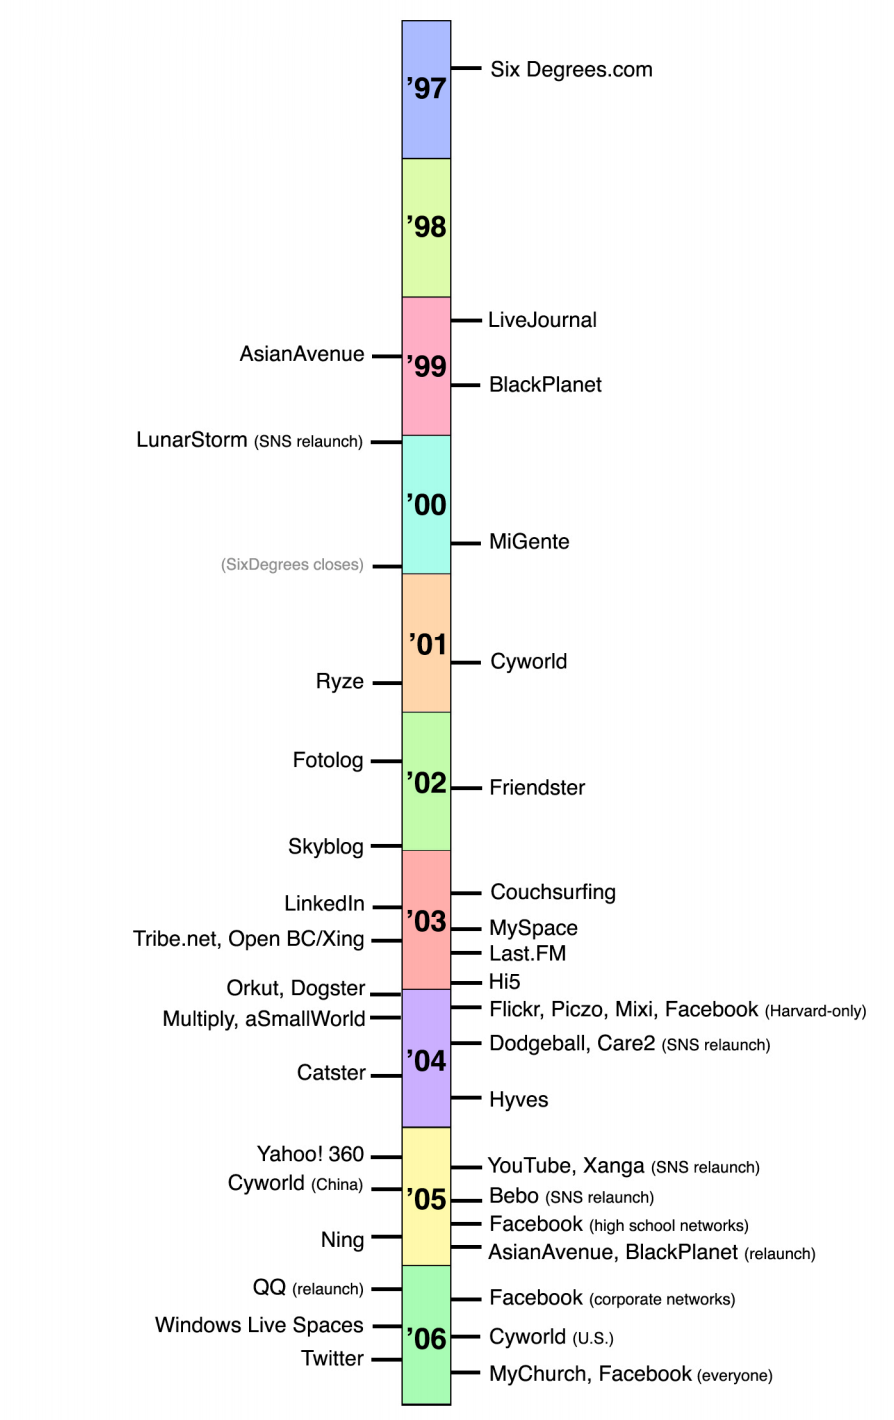
\includegraphics[width=0.7\textwidth]{img/timeline.png}
\end{center}
\caption{\label{img:timeline} Lauch dates of major \glspl{osn}. (\cite{ellison2007social})}
\end{figure}

Although the first platform possessing some of the main characteristics that define \glspl{osn},
according to \cite{ellison2007social}, the first recognizable \gls{osn} launched in 1997 as we can observe in the Figure \ref{img:timeline}. \textit{SixDegrees.com} allowed users to create personal
profiles, connect with friends and consult friends of friends lists. The profile feature came from the
online dating sites and online communities, while the surfing trough register users in the network
and consult friends was an existing feature in Classmates.com. \textit{SixDegrees.com} was the first to combine
these features.

\textit{SixDegrees} promoted itself as a tool to help people to connect, but in 2000, it became an
unsustainable business and the service closed. At the time the creators conclude that
\textit{SixDegrees} was a service that was very ahead of its time.

Until 2002 many \glspl{osn} have emerged, but still incapable of projecting themselves at a global scale.
As we can observe in the timeline of Figure \ref{img:timeline} from 2002 and 2005 the \textit{big players} came to existence, in these period, \gls{osn}
such as Friendster, LinkedIn, MySpace, Hi5, Facebook and Youtube were born, shaping the business, cultural
and research landscape.


%% ---------------------------------------------- Exploring Some OSNs
\section{Exploring Specific Online Social Networks}

In this section we are going to explore in greater detail some of the \glspl{osn} presented
in the Table \ref{table:osns}. The selection of the social networks was not aleatory, we are going
to study deeply the \glspl{osn} that gather some important characteristics, that will be of use in
the future when we design the system for analyzing and visualizing social networks. First, the
\gls{osn} must be accessible, this said, one must be capable of extracting information from the platform
in order to analyze it. Second, in order to obtain large networks, and since this project is being
developed in Portugal, \glspl{osn} that are known to be massively adopted by portuguese (this topic was
addressed in the previous section, where we did an overview to \cite{marktest2016}). Third and at last,
the \glspl{osn} must be the most diversified as possible in terms of their porposes, so that we
can draw different types of conclusions derived from different kind of analysis, for then give proof
of the adaptability of the system to different kinds of \glspl{osn}.\\
\indent This said, these are the following \glspl{osn} that will explored deeply in the proceeding sections:
\begin{itemize}
  \item Facebook
  \item Twitter
  \item LinkedIn
  \item ...
\end{itemize}

\subsection{Facebook}

Facebook allows you to send messages and post status updates to keep in touch with friends and family. You can also share different types
of content, like photos and links. But sharing something on Facebook is a bit different from other types of online communication, because shared content
on facebook is, by default, public.

\subsubsection*{Domain Model}

\begin{figure}[h!]
  \hspace*{-1in}
  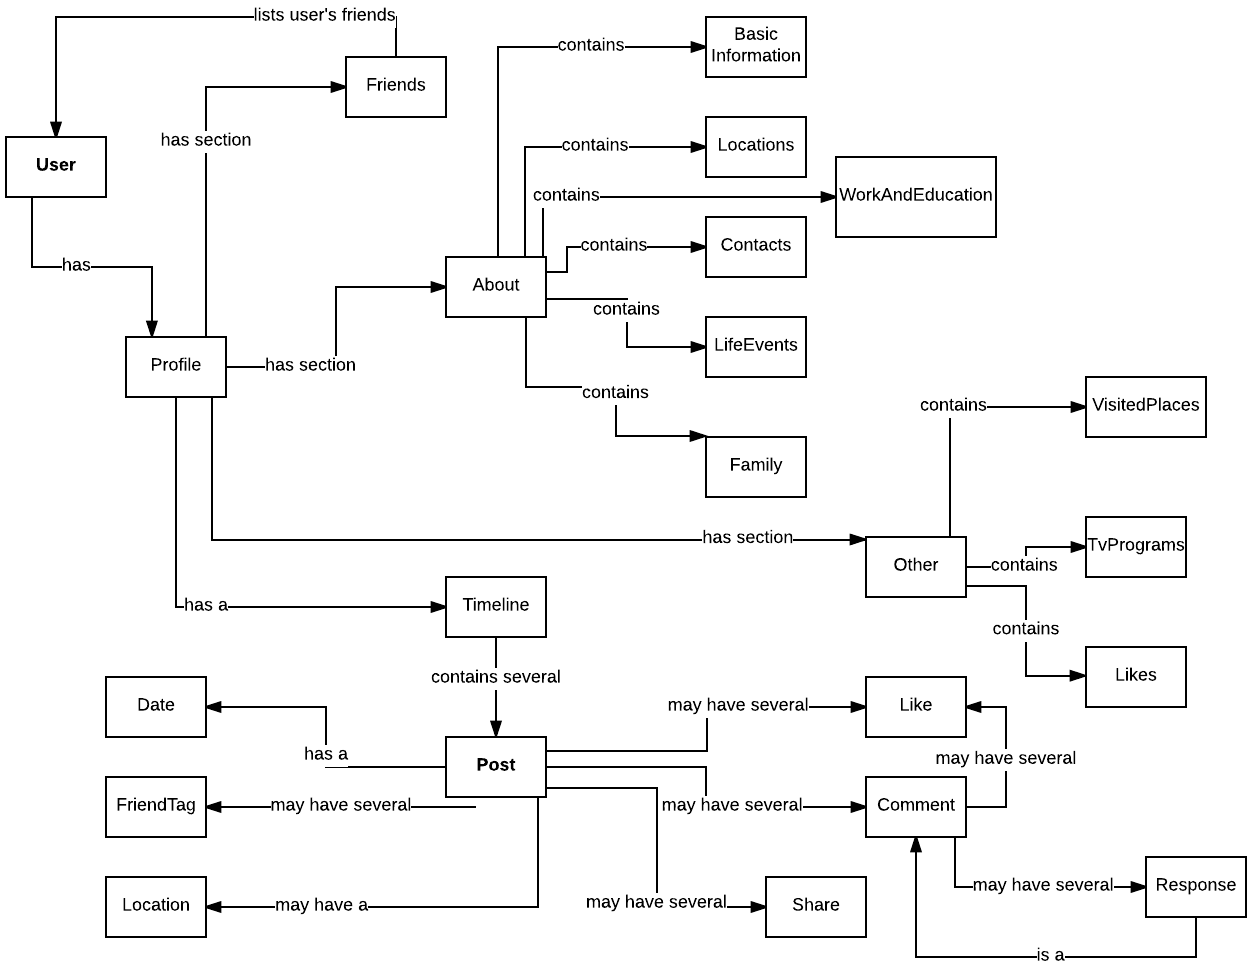
\includegraphics[width=1.2\textwidth]{img/facebook-domain-model.png}
\caption{\label{img:fbdomain} Facebook domain model schema.}
\end{figure}

\indent

\subsubsection*{Facebook Graph API}


%% ---------------------------------------------- How Social Networks Have Changed The World
\section{How Social Networks Have Changed The World}
% Cool overview: https://www.youtube.com/watch?v=trH4iuebjjI
% What really changed? What people did that was good that people don't do anymore? A general overview to the impacts of OSNs!

	
	
	% CHAPTER - Social Network Analysis -------------------------
	\chapter{Social Network Analysis}
	%% ---------------------------------------------- Chapter Introduction

% Social network analysis is the application of network theory to the modeling and analysis of social systems.
% it combine both tools for analyzing social relations and theory for explaining the structures that emerge from the social interactions.
%
% Of course the idea of studying societies as networks is not a new one but with the rise in computation and the
% emergence of a mass of new data sources, social network analysis is beginning to be applied to all type and
% scales of social systems from, international politics to local communities and everything in between.
%
% Traditionally when studying societies we think of them as composed of various types of individuals and organizations,
% we then proceed to analysis the properties to these social entities such as their age, occupation or population, and them ascribe quantitative value to them.
%
% This allows social science to use the formal mathematical language of statistical analyst to compare the values of
%  these properties and create categories such as low in come house holds or generation x, we then search for quasi
%  cause and effect relations that govern these values.
%
% This component-based analysis is a powerful method for describing social systems. Unfortunately though is fails to
% capture the most important feature of social reality that is the relations between individuals, statistical analysis
% present a picture of individuals and groups isolates from the nexus of social relations that given them context.
%
% Thus we can only get so far by studying the individual because when individuals interact and organize, the results
% can be greater than the simple sum of its parts, it is the relations between individuals that create the emergent
% property of social institutions and thus to understand these institutions we need to understand the networks of social relations that constitute them.
%
% Ever since the emergence of human beans we have been building \glspl{sn}, we live our lives embed in networks
% of relations, the shape of these structures and where we lie in them all effect our identity and perception of the world.
%
% A social network is a system made up of a set of social actors such as individuals or organizations and a set of
% ties between these actors that might be relations of friendship, work colleagues or family. Social network science
% then analyze empirical data and develops theories to explaining the patterns observed in these networks
%
% In so doing we can begin to ask questions about the degree of connectivity within a network, its over all structure,
% how fast something will diffuse and propagate through it or the Influence of a given node within the network. lets take some examples of this
%
% Social network analysis has been used to study the structure of influence within corporations, where traditionally
% we see organization of this kind as hierarchies, by modeling the actual flow of information and communication as a
% network we get a very different picture, where seemingly irrelevant employees within the hierarchy can in fact have significant influence within the network.
%
% Researcher also study innovation as a process of diffusion of new ideas across networks, where the oval structure
% to the network, its degree of connectivity, centralization or decentralization are a defining feature in the way
% that innovation spreads or fails to spread.
%
% Network dynamics, that is how networks evolve overtime is another important area of research, for example within Law
% enforcement agencies social network analysis is used to study the change in structure of terrorists groups to identify
% changing relations through which they are created, strengthened and dissolved?
%
% Social network analysis has also been used to study patterns of segregation and clustering within international politics
% and culture, by mapping out the beliefs and values of countries and cultures as networks we can identify where opinions and beliefs overlap or conflict.
%
% Social network analysis is a powerful new method we now have that allows us to convert often large and dense data sets
% into engaging visualization, that can quickly and effectively communicate the underlining dynamics within the system.
%
% By combine new discoveries in the mathematics of network theory, with new data sources and our sociological understanding,
% social network analysis is offering huge potential for a deeper, richer and more accurate understanding, of the complex social systems that make up our world.

\gls{sna} is the study of how people are connected to each other, basically it studies a set of relations among a set of entities,
these entities may be individuals, organizations, or even countries.\\\\
\indent The common analysis procedure consists in mapping the network and then create metrics to
characterize the network. Then one tries to figure what is the structure of the network and why does
it have that structure. \gls{sna} is also about look at the individuals inside the network and where are those individuals located.

\section{Fundamental Concepts for Network Analysis}

The concepts listed below are of key importance to understand \gls{sna}.\cite{wasserman1994social}

\begin{itemize}
    \item \emph{Actor} - \gls{sna} is concerned with understanding the linkages among social entities and the implications of these linkages, these social entities are described as actors. Actors are are discrete individual, corporate, or collective social units.
    \item \emph{Relational Tie} - Actors are linked to one another trough \textit{social ties}. The type of ties may be extensive, and it describes the nature of the connection. Some example of ties:
        \begin{itemize}
            \item \textbf{Evaluation} of one person by another;
            \item \textbf{Transference} of resources (business transactions);
            \item \textbf{Association} (to social event or cause);
            \item \textbf{Behavioural} interactions (communicating);
            \item \textbf{Moving} between places or statuses (migration, social or physical mobility);
            \item Others may be: physical connection (roads, rivers), formal relations (authority), biological relationship;
        \end{itemize}
    \item \emph{Dyad} - The most basic relationship that can be established is a dyad, a connection between two actors.
    \item \emph{Triad} - A relation established between three actors. Many studies included breaking \glspl{sn} down to small groups (triads), this allowed a more clear conclusion about the transitivity of the connections.
    \item \emph{Subgroup} - It defines any subset of actors in a \gls{sn} (conceptually, subgroups come after dyads and triads).
    \item \emph{Group} - A finite set of actors who for conceptual, theoretical or empirical reasons are treated as a finite set of individuals in which network measurements are made.
    \item \emph{Relation} - A collection of ties of a specific kind among members of a group is called a \textbf{relation} (e.g. a connection in \textit{LinkedIn} is a relation while evaluating our connections of sending them messages are ties).
    \item \emph{\gls{sn}} - With the definitions of actor, group and relation, a \gls{sn} consists of a finite set or sets of actors and
    and the relation or relations defined on them. The presence of relation information is critical and defining feature of a \gls{sn}.
\end{itemize}

\section{Network Analysis}
\subsection{Scientific Background}
\subsection{Graphs Theory}
\subsection{Statistics}
\subsection{...}
\subsection{Power Law}
\subsection{Centrality Measures}
\subsection{Community Detection}
\subsection{Spread of Information}
\subsection{Link Analysis}
\subsection{...}
\section{Six Degrees of Separation}
% Small World Problem, Stanley Milgram's Experiment

\section{Network Visualization}
% It's a science by itself. REF ao documento STAR report on Dynamic Graph Visualization

\section{Real World Applications}
% What SNAs are used for.

\section{Social Network Analysis Software}

	
	\section{Network Visualisation}
	% It's a science by itself.
	
	\section{Real World Applications}
	% What SNAs are used for.


	% CHAPTER - Problem and Challenges ---------------
	\chapter{The problem and its challenges}


	% CHAPTER - Proposed Solution -------------------------
	\chapter{Proposed Solution}
	\section{Solution Requirements}
	\subsection{Requirements Analysis}
	\subsection{Requirements Specification}
	\subsection{Requirements Prioritisation}
	\section{System Modeling}
	\section{System Architecture}
	\section{Technology Selection}
	\subsection{Technology A}
	\subsection{Technology B}
	\subsection{Technology C}
	\subsection{Technology Comparison}
	\subsection{Decision}
	
	
	% CHAPTER - Implementation -------------------------
	\chapter{Implementation}
	\section{Data Extraction}
	\subsection{Data Sources} % Related to Online Social Networks Chapter
	\section{Data Mining}
	\section{Back end}
	\section{Front end}
	\section{Outcomes}


	% CHAPTER - Results -------------------------
	\chapter{Case Studies}
	Application of main result (examples and case studies)
    	\section{Results}
    	\section{Discussion}
	\section{Summary}

	% CHAPTER - Conclusion/Future Work --------------
	\chapter{Conclusion}
	Conclusions and future work.
	\section{Conclusions}
	\section{Prospect for future work}
			
	\bookmarksetup{startatroot}
	\addtocontents{toc}{\bigskip}
	\cleardoublepage

	%- Bibliography (needs bibtex) -%
	\bibliography{dissertation}

\end{document}
